\subsection{Overview}
\label{sec:ovw}

We now briefly describe the approach. Given a numerical simulator
$\simulate$ and an initial abstraction defined by a quantization
function $\quant_\epsilon$ and a time step $\Delta$, we use
scatter-and-simulate (parameterized by number of samples $n$ as
described in \chapref{abs}) to explore the abstract graph
$\scr{H}(\Delta)$. The result is a graph $G$, which has a finite
number of abstract states $C$ (or cells) and edges $(C,C')$ iff $C
\areach{\Delta} C'$.

Instead of using a CEGAR like loop (as in \chapref{abs}), we use the
generated trajectory segments to learn quantitative models describing
the local behavior of the system. These models are defined by a set of
relations $R \subseteq \HybridStates \times \HybridStates$ for each
edge of the reachability graph.


\begin{figure}[!htbp]
\begin{center}
\tikzstyle{line} = [thick]
\tikzstyle{arw} = [->, thick,>=stealth,shorten <=2pt, shorten >=2pt]
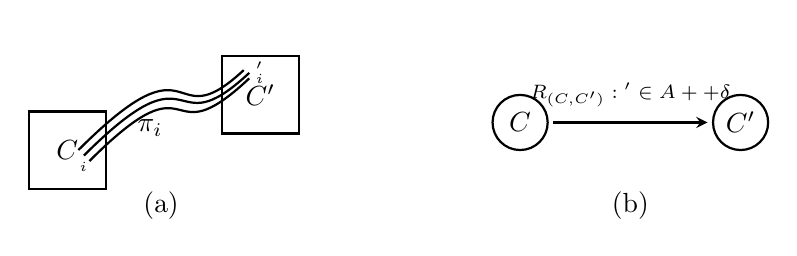
\begin{tikzpicture}
\begin{scope}[scale=0.7]

    \draw [line] (-5.2,-1.2) rectangle (-3.8,0.2);
    \draw [line] (-1.7,-0.2) rectangle (-0.3,1.2);
    \draw [line] (-4.1,-0.7) .. controls +(2.0,2.0) and +(-1.6,-1.5) ..  (-1.2,0.8);
    \draw [line] (-4.2,-0.6) .. controls +(2.1,2.1) and +(-1.5,-1.4) ..  (-1.2,0.9);
    \draw [line] (-4.3,-0.5) .. controls +(2.2,2.2) and +(-1.4,-1.3) ..  (-1.3,0.95);

\node at (-4.5, -0.5) {$C$};
\node at (-1, 0.5) {$C'$};
\node at (-4.2,-0.8) {\scriptsize{$\x_i$}};
\node at (-1.0,0.90) {\scriptsize{$\x_i'$}};
\node at (-3,-0.1) {$\pi_i$};
\node at (-2.8, -1.5) {(a)};
\end{scope}

\begin{scope}[xshift=4.0cm,scale=0.7]
\draw [line] (-2.0,0) circle (0.5);
\draw [line] (2.0,0) circle (0.5);
\draw[arw] (-1.5,0) -- (1.5,0);
\node at (-2.0,0) {$C$};
\node at (2.0,0) {$C'$};
\node at (0,0.5) {\scriptsize{$R_{(C,C')}:\setof{\x' \in A\x + \vb + \delta}$}};
\node at (0.,-1.5) {(b)};
\end{scope}
\end{tikzpicture}
\end{center}
\vspace*{-.3cm}
\caption{(a) Trajectory segments $\traj_i$ are used to compute the
relation $R_{(C,C')}$ that annotates the edge in (b).
$R_{(C,C')}:\setof{\x' \in A\x + \vb + \delta}$ is an interval affine
relation defined by an affine map (matrix $A$ and vector $\vb$) and an
error interval (vector of intervals $\delta$).}
    \label{fig:enriched-edge}
\vspace*{-.3cm}
 \end{figure}


Recall that each edge $(C,C')$ of the graph $G$ denotes an observed
trajectory segment between the respective cells. The graph abstraction
$G$ only states that there exists a state $\x \in C$ from which the
system can evolve to a future state $\x' \in C'$. To increase the
precision we iteratively refined the abstraction by state
splitting. Instead, we now propose an `enrichment' $G^R$ of $G$ by computing a
set of local relations $R_{(C,C')}(\x,\x')$ for every edge $(C,C')$,
which non-deterministically describe relations between $\x \in C$ and $\x'
\in C'$. This is illustrated in \figref{enriched-edge} (compare with
\figref{segtraj}).

The enriched graph $G^R$ captures the underlying local forward
dynamics describing the evolution of the system in each abstract
state. We represent the dynamics using an affine model with an
interval error. Such a model can either be approximated using learning
methods or computed as a sound (over) approximation using reachability
set computation methods. Because we assume black box semantics, we
only present the former. Using regression analysis on the $start$ and
$end$ states of the witnessed trajectory segments between two cells,
we compute an approximate discrete map along with an error estimate.
Moreover, using the simulation function $\simulate$, additional
trajectory segments (or data) can be generated if required. The data
can be separated into a training set and testing set to compute the
map and the error respectively.  The latter case can be explored if
the symbolic dynamics of the system are known. A tool like
\flowstar~\cite{chen2013flow} can be used to find the reachable set
map.

Observe that $G^R$, a directed reachability graph, is rich enough to
search for concrete behaviors in the system. We call it a time
parameterized PWA relational abstraction. It can be interpreted as an
infinite state discrete transition system, and we can use
off-the-shelf bounded model checkers to find concrete violations of a
given safety property, and even other temporal properties.  We now
discuss the background required to present our ideas.
